\clearpage
\subsection{Smooth nonconvex and matched-noise controls}
\label{app:nonconvex-empirical}
The existing nonconvex campaign supplies a smooth SGD construction with a
proved invariant law and separately measured positive tangent growth.
Its batch loss is
\[
 L_B(x)=\frac{h_Bx^2}{2}-\xi_Bx
        -\frac{0.92}{2}\bigl[x^2-\log(1+x^2)\bigr],
 \qquad
 \xi_B\mid h_B\sim\mathcal N(0,\sigma^2h_B/B),
\]
where $h_B$ averages $B$ independent equiprobable values $0.95$ and $1.05$.
Every sampled loss is coercive, but the population Hessian attains $-0.035$.
The exact update is
\[
 x^+=[1-\eta(h_B-0.92)]x
           -\frac{0.92\eta x}{1+x^2}+\eta\xi_B.
\]
At $\eta=8$, the outer coefficient lies in $[-0.04,0.76]$ and the nonlinear
remainder is bounded. Global drift and Gaussian minorization therefore give a unique
attracting invariant law with every polynomial moment finite, independently
of the numerical tangent calculation.
The reference at $x=0$ has log gain $1.94427$ and harmonic gain $6.97714$.
Three completed FP64 configurations, each with 16 chains and one million updates,
give mean moving log growth $+0.18959$ for $B=1$, $\sigma=0.001$.
These finite-horizon measurements suggest positive long-time growth but do not
prove the smooth model's infinite-time exponent; the positive stationary exponent
of the piecewise control in the main text is established analytically.

\begin{figure}[!ht]
\centering
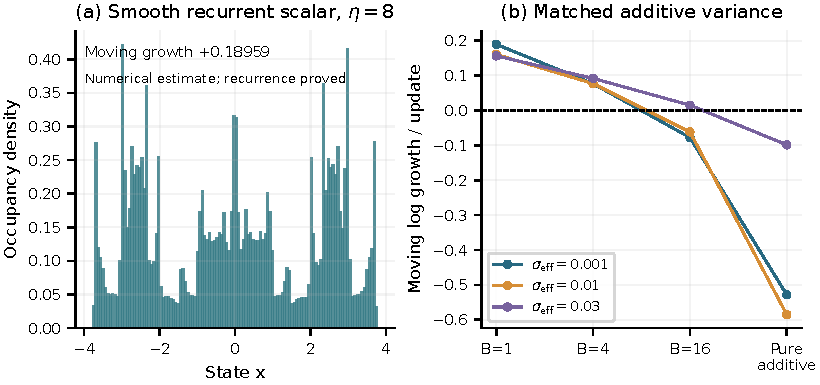
\includegraphics[width=\linewidth]{figures/empirical_nonconvex_scalar_controls.pdf}
\caption{\textbf{Smooth recurrence and a controlled multiplicative-noise intervention.}
(a) Pooled occupancy from all saved 20,000-update dense followups to the three
million-update, 16-chain FP64 confirmations at $\eta=8$, $B=1$, $\sigma=0.001$.
The density is multimodal; no exactly-two-mode claim is made.
The displayed moving growth is estimated from the primary long trajectories.
(b) A separate intervention sets the per-example residual scale to
$\sigma_{\rm eff}\sqrt B$, so that
$\operatorname{Var}(\xi_B)=\sigma_{\rm eff}^2$ stays fixed while
$\operatorname{Var}(h_B)=0.0025/B$ changes.
Points average completed million-update configurations; the pure-additive control sets $h_B=1$.
Thus batching can change the moving-growth sign even with matched unconditional additive variance.}
\label{fig:nonconvex-scalar-controls}
\end{figure}

The matched-variance results distinguish the two sources of randomness:
at $\sigma_{\rm eff}=0.001$, moving growth changes from $+0.18917$ at $B=1$
to $-0.07775$ at $B=16$, whereas the pure-additive control gives $-0.52845$.
Conditional dependence between $h_B$ and $\xi_B$ remains as specified; matching
variance does not make them independent.
The finite-time means, correlated occupancy samples, and local density shape do not
prove the sign of an asymptotic tangent exponent or a universal harmonic-to-bimodal transition.

\clearpage
\subsection{Constructed neural recurrence versus ordinary-network controls}
\label{app:constructed-vs-ordinary}
The constructed networks have two or four affine layers, hidden width four,
and tanh or sigmoid activations, fitted to 64 fixed inputs sampled uniformly from $[-1,1]^2$,
with targets $\sin(3x_1)+0.7x_1x_2+0.3\cos(4x_2)$.
Effective weights and biases are bounded transforms of unconstrained latent parameters:
$W=(2/\sqrt{\mathrm{fan\_in}})\tanh\theta_W$, $b=\tanh\theta_b$.
Their sampled objective is
\[
 \frac1{2B}\sum_{i\in I}(f_\theta(x_i)-y_i)^2
 +\frac\mu2\|\theta\|^2-\sigma_{\rm eff}z^\top\theta,
 \qquad z\sim\mathcal N(0,I).
\]
Here the data gradient is globally bounded and the latent update has outer
coefficient $1-\eta\mu$; with $\mu=0.05$ and $\eta\in\{0.5,10\}$, recurrence
with all moments follows from the global return argument.
The full-rank parameter-linear forcing is an explicit design choice, distinct from regression label noise.
Freezing the output bias restricts the state and forcing to the remaining active coordinates.

\begin{figure}[!ht]
\centering
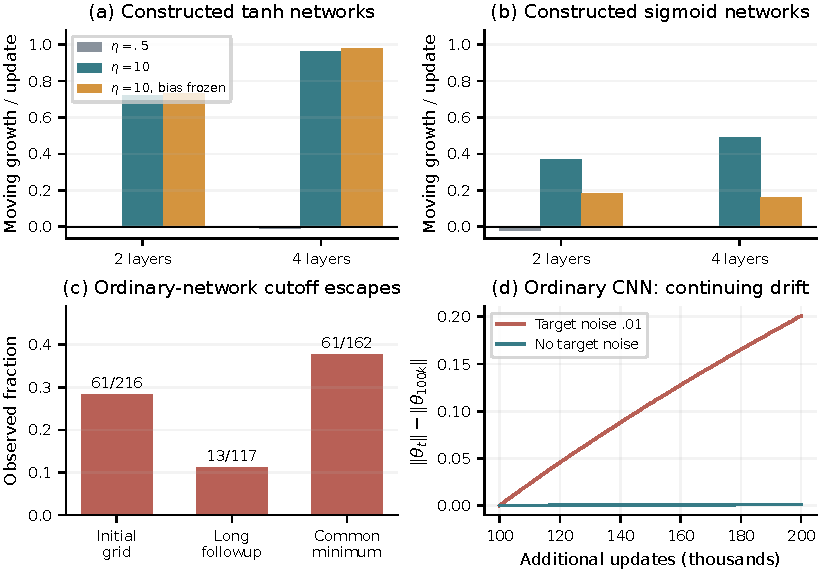
\includegraphics[width=\linewidth]{figures/empirical_nonconvex_network_controls.pdf}
\caption{\textbf{Constructive positive controls do not imply ordinary-network equilibrium.}
(a,b) At $B=8$, $\sigma_{\rm eff}=0.003$, moving-growth means use the final
500,000 updates of completed million-update constructed-network confirmations, with 48 chains per setting.
Large-step positive growth survives the frozen-output-bias ablation; four-layer tanh gives
$+0.96022$ with trainable bias and $+0.97751$ with frozen bias.
These are numerical growth estimates in models with separately proved recurrence.
(c) The ordinary-network campaign retains all 495 completed cells, including
135 loss-cutoff escapes; cohorts have different designs and horizons, so these fractions
are not a controlled comparison of escape probabilities.
(d) A separate ordinary CIFAR-10 CNN at $\eta=0.08$, $B=128$ continues to drift
over 200,000 additional updates. The displayed noisy and noiseless paths share
their parent checkpoint and minibatch stream. A finite path's norm drift does not
measure ensemble-variance growth or prove mathematical escape.}
\label{fig:nonconvex-network-controls}
\end{figure}

In the matched CNN pair, the norm-mean shift between updates
$[100000,150000)$ and $[150000,200000)$ is $0.10005$ with target-noise
standard deviation $0.01$, versus $0.000613$ without added noise.
Its tiny float32 moving-growth signs are unresolved and are not used to claim an invariant law.
The broader ordinary controls include continuing parameter drift and dead-feature ReLU states
whose remaining output bias follows a stable scalar recursion; these are not sustained
positive-tangent neural equilibria.
All figures use completed executions. The prospective next-study protocol contributes no results or counts.
\clearpage
